%%%%%%%%%%%%%%%%%%%%%%%%%%%%%%%%%%%%%%%%%
% Arsclassica Article
% LaTeX Template
% Version 1.1 (1/8/17)
%
% This template has been downloaded from:
% http://www.LaTeXTemplates.com
%
% Original author:
% Lorenzo Pantieri (http://www.lorenzopantieri.net) with extensive modifications by:
% Vel (vel@latextemplates.com)
%
% License:
% CC BY-NC-SA 3.0 (http://creativecommons.org/licenses/by-nc-sa/3.0/)
%
%%%%%%%%%%%%%%%%%%%%%%%%%%%%%%%%%%%%%%%%%

%----------------------------------------------------------------------------------------
%	PACKAGES AND OTHER DOCUMENT CONFIGURATIONS
% Author: Changgang Zheng
% E-mail: changgangzheng@foxmail.com
%----------------------------------------------------------------------------------------
\documentclass[
12pt, % Main document font size
a4paper, % Paper type, use 'letterpaper' for US Letter paper
oneside, % One page layout (no page indentation)
%twoside, % Two page layout (page indentation for binding and different headers)
headinclude,footinclude, % Extra spacing for the header and footer
BCOR5mm, % Binding correction
]{scrartcl}
\usepackage{cite}
\usepackage{pdfpages}
%%%%%%%%%%%%%%%%%%%%%%%%%%%%%%%%%%%%%%%%%
% Arsclassica Article
% Structure Specification File
%
% This file has been downloaded from:
% http://www.LaTeXTemplates.com
%
% Original author:
% Lorenzo Pantieri (http://www.lorenzopantieri.net) with extensive modifications by:
% Vel (vel@latextemplates.com)
%
% License:
% CC BY-NC-SA 3.0 (http://creativecommons.org/licenses/by-nc-sa/3.0/)
%
%%%%%%%%%%%%%%%%%%%%%%%%%%%%%%%%%%%%%%%%%

%----------------------------------------------------------------------------------------
%	REQUIRED PACKAGES
%----------------------------------------------------------------------------------------

\usepackage[
nochapters, % Turn off chapters since this is an article
beramono, % Use the Bera Mono font for monospaced text (\texttt)
eulermath,% Use the Euler font for mathematics
pdfspacing, % Makes use of pdftex’ letter spacing capabilities via the microtype package
dottedtoc % Dotted lines leading to the page numbers in the table of contents
]{classicthesis} % The layout is based on the Classic Thesis style

\usepackage{arsclassica} % Modifies the Classic Thesis package

\usepackage{geometry}
\geometry{left=3.0cm,right=3.0cm,top=3.0cm,bottom=3.0cm}


\usepackage[T1]{fontenc} % Use 8-bit encoding that has 256 glyphs

\usepackage[utf8]{inputenc} % Required for including letters with accents

\usepackage{graphicx} % Required for including images
\graphicspath{{Figures/}} % Set the default folder for images

\usepackage{enumitem} % Required for manipulating the whitespace between and within lists

\usepackage{lipsum} % Used for inserting dummy 'Lorem ipsum' text into the template

\usepackage{subfig} % Required for creating figures with multiple parts (subfigures)

\usepackage{amsmath,amssymb,amsthm} % For including math equations, theorems, symbols, etc

\usepackage{varioref} % More descriptive referencing

%----------------------------------------------------------------------------------------
%	THEOREM STYLES
%---------------------------------------------------------------------------------------

\theoremstyle{definition} % Define theorem styles here based on the definition style (used for definitions and examples)
\newtheorem{definition}{Definition}

\theoremstyle{plain} % Define theorem styles here based on the plain style (used for theorems, lemmas, propositions)
\newtheorem{theorem}{Theorem}

\theoremstyle{remark} % Define theorem styles here based on the remark style (used for remarks and notes)

%----------------------------------------------------------------------------------------
%	HYPERLINKS
%---------------------------------------------------------------------------------------

\hypersetup{
%draft, % Uncomment to remove all links (useful for printing in black and white)
colorlinks=true, breaklinks=true, bookmarks=true,bookmarksnumbered,
urlcolor=webbrown, linkcolor=webgreen, citecolor=webgreen, % Link colors
pdftitle={}, % PDF title
pdfauthor={\textcopyright}, % PDF Author
pdfsubject={}, % PDF Subject
pdfkeywords={}, % PDF Keywords
pdfcreator={pdfLaTeX}, % PDF Creator
pdfproducer={LaTeX with hyperref and ClassicThesis} % PDF producer
}
 % Include the structure.tex file which specified the document structure and layout
\usepackage{newpythonhighlight}
\usepackage{listings}
\lstset{
language=bash,
xleftmargin=1.8em
}
\usepackage[numbered, autolinebreaks,useliterate]{mcode}
\usepackage{xcolor}
\usepackage{color}
\usepackage[utf8]{inputenc}
\usepackage[T1]{fontenc}
\usepackage{mathrsfs,amsmath}
\usepackage{amssymb}
\usepackage{bm}
\usepackage{longtable}
\usepackage{algorithmic}
\usepackage[ruled,linesnumbered]{algorithm2e}

\hyphenation{Fortran hy-phen-ation} % Specify custom hyphenation points in words with dashes where you would like hyphenation to occur, or alternatively, don't put any dashes in a word to stop hyphenation altogether

%----------------------------------------------------------------------------------------
%	TITLE AND AUTHOR(S)
%----------------------------------------------------------------------------------------
\title{\normalfont\spacedallcaps{Final Report}} % The article title
%\subtitle{Subtitle} % Uncomment to display a subtitle
%\author{\spacedlowsmallcaps{Changgang Zheng\textsuperscript{1}}} % The article author(s) - author affiliations need to be specified in the AUTHOR AFFILIATIONS block
%\date{} % An optional date to appear under the author(s)
%----------------------------------------------------------------------------------------
\begin{document}
% 
\includepdf[pages=-2]{top.pdf}
%
\includepdf[pages=-1]{cover.pdf}
%----------------------------------------------------------------------------------------
%	HEADERS
%----------------------------------------------------------------------------------------
\renewcommand{\subsectionmark}[1]{\markright{\spacedlowsmallcaps{#1}}} % The header for all pages (oneside) or for even pages (twoside)
%\renewcommand{\subsubsectionmark}[1]{\markright{\thesubsection~#1}} % Uncomment when using the twoside option - this modifies the header on odd pages
\lehead{\mbox{\llap{\small\thepage\kern1em\color{halfgray} \vline}\color{halfgray}\hspace{0.5em}\rightmark\hfil}} % The header style

\pagestyle{scrheadings} % Enable the headers specified in this block

%----------------------------------------------------------------------------------------
%	TABLE OF CONTENTS & LISTS OF FIGURES AND TABLES
%----------------------------------------------------------------------------------------
%\maketitle % Print the title/author/date block

\thispagestyle{empty}
\setcounter{tocdepth}{3} % Set the depth of the table of contents to show sections and subsections only


%\let\thefootnote\relax\footnotetext{1\textit{Glasgow College, University of Electronic Science and Technology of China, ChengDu, China}}

%\tableofcontents % Print the table of contents

\thispagestyle{empty}
%\listoffigures % Print the list of figures
% \listoftables % Print the list of tables
\newpage




%----------------------------------------------------------------------------------------
%	AUTHOR AFFILIATIONS
%----------------------------------------------------------------------------------------

\setcounter{page}{1}

\subsection{Environment System Construction}
\noindent Environment is defined in four layers, with three 2-dimensional Gaussian distillation layers and one uniform distribution layer. For Gaussian distributed layers, 300, 250 and 200 MSs follows a 10, 7 and 6 meters standard deviation respectively, and their mean are randomly distributed. Also, following 300 MSs follow a uniform distribution. After adding them all together. For an unbiased comparison environemnt, the random seed is fixed. All the following plots are running on the same environment.\\
\begin{figure}[h]%%图
	\centering  %插入的图片居中表示
	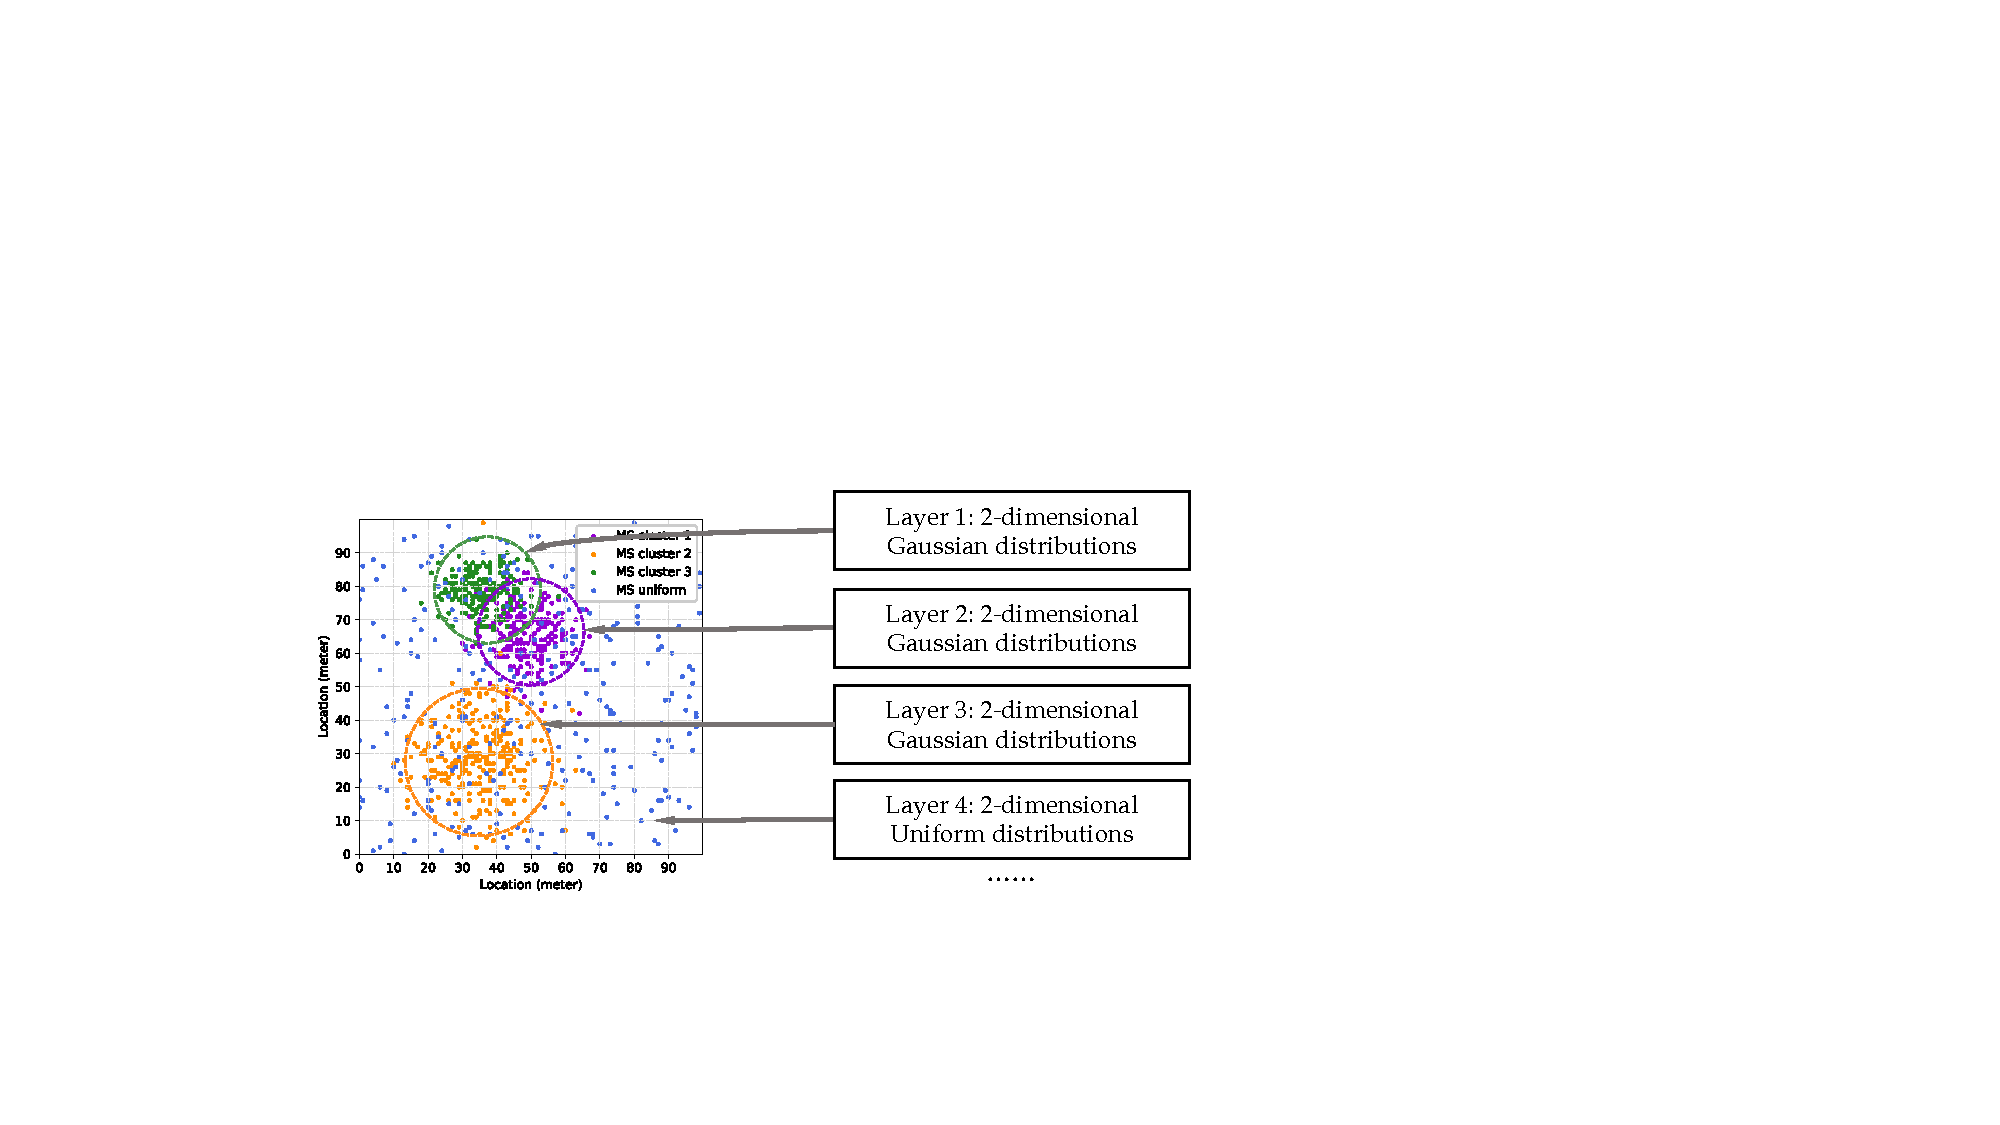
\includegraphics[width=0.8\linewidth]{figures/env_cons}  %插入的图,包括JPG,PNG,PDF,EPS等,放在源文件目录下
	\caption{Environment construction}  %图片的名称
	\label{fig:env_cons}   %标签,用作引用
\end{figure}




\subsection{Communication System Construction}
Signal to Interference Plus Noise Ratio and Reference Signal Received Power, which are used for evaluating the potential signal quality between Airborne-BSs and users' device. And a threshold (40dB) is proposed to distinguish the connection states.\\
\begin{equation}
R S R P_{n, u}= \frac{EIRP}{L_{\mathrm{s}}}= \frac{EIRP\; c^{2}}{\left(4\pi  f_{\mathrm{c}} d\right)^{2}}
\label{rsrp}
\end{equation}
\noindent The RSRP for the link between user $u$ and Airborne-BS $n$ is calculated according to the EIRP, and free space path loss is given in Equation \ref{loss}.
\begin{equation}
S I N R_{n, u}=\frac{R S R P_{n, u}}{N+\sum_{\forall i \neq n} R S R P_{i, u}}
\label{sinr}
\end{equation}
\noindent Signal to Interference plus Noise Ratio (SINR) is given in Equation \ref{sinr}, where $N$ is the noise power in Watts.



\subsection{Training and Results}
\noindent The Q-Learning, SARSA, DQN are firstly tested in our environment. In this interim report, the SARSA and Q-Learning is evaluated, and DQN will be implemented in the following experiment. During the experiment, SARSA and Q-Leaning are tested in an even parameter space with the leaning rate $\alpha = 0.1$, the discount factor $\lambda=0.9$ and the greedy policy $\epsilon=0.9$. The leaning includes 100 episode, where 2000 steps are in either of it. For each step, every Airborne-BS can do a single action, including 'east', 'west', 'south', 'north' and 'stay'. When beginning a new episode, the Airborne-BSs are settled back to the initial position. The initial points of the Mobile Stations are set with a fixed random seed for different algorithm. And the Airborne-BSs' initial position are evenly distributed in the four corners and sides of the environment. \\

\begin{algorithm}
	\caption{DQN implementation}
	\label{alg2}
	\begin{algorithmic}[1]
		\STATE Initialization
		\FOR{every episode $j$}
    \STATE $s_{1} \leftarrow \text { random }$
		\FOR{$\text {Every iteration } t$}
    \FOR{$\text { Every drone } \delta$}
    \STATE $ a_{t}\leftarrow \max _{a} Q\left(\phi\left(s_{t}\right), a ; \theta\right)\text { with probability } \epsilon \text { select a random action } $
    \STATE $ r_{t}, x_{t+1} \leftarrow \text { based on the action } \mathrm{a}_{t}$
		\STATE $\phi_{t+1}=\phi\left(s_{t+1}\right)\leftarrow s_{t+1}=\left(s_{t}, a_{t}, x_{t+1}\right)$
		\STATE $D \leftarrow \text { Add data to the dataset } D+\left(\phi_{t}, a_{t}, r_{t}, \phi_{t+1}\right)$
    \STATE $ eva Q_{t+1} \leftarrow \text {evaQ learn from data selected in } D$
    \STATE $s_{t} \leftarrow \mathrm{s}_{t+1} $
    \ENDFOR
		\STATE $ Q \leftarrow \text{ fine-tune the parameters from }  evaQ \text{ for every n steps} $
		\ENDFOR
		\ENDFOR
	\end{algorithmic}
\end{algorithm}







%\bibliographystyle{IEEEtran}
%\bibliography{reference/ref.bib}
\end{document}
